\documentclass{article}
\usepackage{graphicx}
\usepackage{float}
\usepackage{microtype}
\usepackage{textcomp, gensymb}
\begin{document}
\section{Week 1: Vector Analysis}
\subsection{Basic Vector Operations}
The use of vectors is integral to the mathematical modeling of electromagnetic fields and waves; as such, a review of vector analysis, including basic operations, vector calculus, and the use of three common coordinate systems, will come in handy.

First, a refresher on terminology. \textbf{Scalars} represent singular quantities with some magnitude, such as temperature, distance or voltage; \textbf{vectors}, on the other hand, have magnitude and direction, and represent quantities such as heat flow, velocity, (the "vector" versions of temperature and direction) and current.

The magnitude of a vector corresponds with our intuitive sense of "length", and a \textbf{unit vector} refers to a vector with a magnitude of $1$. The rectangular or Cartesian coordinate system consists of the x, y, and z axes, with corresponding unit vectors $\hat{x}$, $\hat{y}$, and $\hat{z}$. These are simply unit vectors that along the direction of their respective axes. Any vector can be reduced to a unit vector by means of the formula $\hat{a} = \frac{\vec{A}}{|A|}$, and doing so leaves behind just the directional component of the associated vector.

Vectors are commonly represented in terms of their components along these different axes. In the rectangular coordinate system, a vector $\vec{A}$ can be represented as $\hat{x}A_{x} + \hat{y}A_{y} + \hat{z}A_{z}$, representing "how much" of the vector points in the direction of each axis. Using basic trigonometry, the magnitude of any such vector $\vec{A}$ in a rectangular coordinate system can be found as $\sqrt{A_x^2 + A_y^2 + A_z^2}$.

Vectors themselves can be operated on much as scalars can be. Starting with the simplest operations, vector addition is performed by adding "matching" components; e.g., $\vec{A} + \vec{B} = \hat{x}(A_{x}+B_{x}) + \hat{y}(A_{y}+B_{y}) + \hat{z}(A_{z}+B_{z})$, while vector subtraction is performed as $\vec{A} + (-\vec{B})$. 

Vector multiplication can be broken into three related operations: scalar multiplication, dot products, and cross products. Scalar multiplication operates solely on the magnitude of a vector, and, as the name implies, is performed by multiplying a scalar with a vector; e.g., $a\vec{A}$ simply multiplies each of the vector $\vec{A}$'s components by $a$ (scalar division works the same way), and returns a vector.

The dot product of two vectors, defined as $\vec{A} \dot \vec{B} = |A|\space|B|cos{\theta_{AB}}$, represents the degree to which the two vectors point in the same direction (a quick way to verify this is to focus on the cosine function: the dot product will be maximized when the angle between the two vectors is $0\degree$, and will equal zero when the angle between the two vectors is $90\degree$). The most immediate application of dot products is to project some vector $\vec{A}$ onto one of the axes unit vectors to determine "how much" of the vector points in that axis' direction. For example, considering a vector $\vec{A}$ that sits on the x-y plane at a $45\degree$ angle, the dot product $\vec{A} \dot \hat{x} = |A|\space|\hat{x}|cos(45\degree) = |A|\space0.707$, corresponding to our intuitive understanding of trigonometric functions/ratios. Dot products take in two vectors and output a scalar.

NOTE: It's interesting to me that a the cosine/sine of a $45\degree$ angle is 0.707, that is, the RMS value of a sinusoidal signal. There is likely some incredibly obvious reason this is the case, which I will think of once this class is over and the information is no longer useful to me. Also, I still don't quite understand the significance of a dot product when one of the vectors is not a unit vector -- I've been told I'll understand this better as we work our way through the course.

The cross product, on the other hand measures the degree to which two vectors are \textit{not} aligned, and is defined by $\vec{A} \times \vec{B} = |A|\space|B|sin(\theta_{AB})\hat{n}$, where $\hat{n}$ is the unit vector pointing towards or away from $\vec{A}$ and $\vec{B}$, as defined by the right-hand rule. (Cyclic relations also help to clarify the direction of the resultant vector). Cross products, like dot products, take in two vectors, but return another vector rather than a scalar.

As a final note, any point on the coordinate plane can be given in terms of its position vector $\vec{OP_1}$, which measures its distance from the origin, or as a distance vector $\vec{P_1P_2} = {P_2 - P_1}$, which measures its distance from another vector.

\subsection{Coordinate Systems}
The most useful coordinate systems in the analysis of fields and waves are the rectangular (Cartesian), cylindrical, and spherical systems. It is important to be able to convert between the coordinate systems and relate the given quantities to each other. Note that all coordinate systems considered here are orthogonal; that is, the unit vectors in the system are mutually perpendicular, at a $90\degree$ angle to each other (meaning their dot product is $0$).

The rectangular (Cartesian) coordinate system, which we have covered briefly is the most familiar one, given in three dimensions by the $x$, $y$, and $z$ axes. The unit vectors in the rectangular coordinate system are $\hat{x}$, $\hat{y}$, and $\hat{z}$, and they are independent of the point given (this will make more sense as we move on to cylindrical and spherical coordinates). 

In the cylindrical coordinate system, we consider a cylinder with radius $r$ centered at the origin, and locate our points at the boundary of this cylinder (see Fig 1). The resultant position vector sits at a distance of $r$ from the origin \textbf{in the x-y plane}, and at a "height" of $z$ (identical to the rectangular system on this plane). However, since this can still describe any point found in a circle at the cylinder's boundary, we use the parameter $\phi$ to describe it's position in reference to an angle beginning at the x-axis and rotating along the cylinder's boundary (thus it has a range of $0 \leq \phi \leq 2\pi$). Any point in this system can be mapped to the x-y-z plane by means of transformations. An exhaustive list of transformations between systems is found in the textbook, but Fig. 2 may help to visualize these transformations.

\begin{figure}[h]
	\centering
	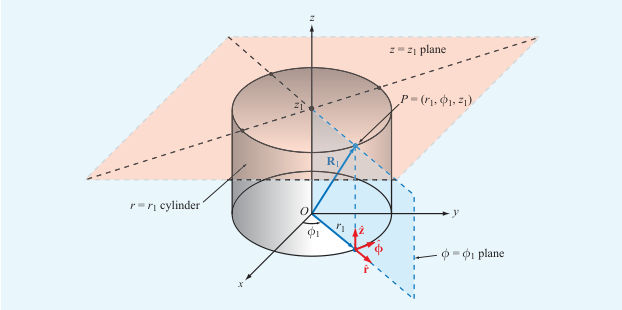
\includegraphics[width=1\textwidth]{fig_1.png}
	\caption{The cylindrical coordinate system.}
	\label{fig:figure 1}
\end{figure}

\begin{figure}[h]
	\centering
	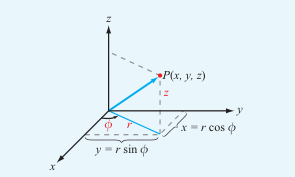
\includegraphics[width=0.6\textwidth]{fig_2.png}
	\caption{Mapping the cylindrical coordinate system onto the rectangular coordinate system.}
	\label{fig:figure 2}
\end{figure}

In the cylindrical coordinate system, unit vector $\hat{z}$ is identical to its rectangular counterpart, while unit vector $\hat{r}$ depends on $\phi$, since this angle will determine the direction $\hat{r}$ points in the x-y plane. $\hat{\phi}$ is the unit vector pointing tangent to the cylinder's boundary at the given point.

In the spherical coordinate system, two angles $\theta$ and $\phi$ are given, along with a raidal component $R$ (it's important that this parameter is distinguished from $r$ in cylindrical components). As the name implies, the spherical coordinate system locates its points on the boundary of a sphere with raidus $R$, with $\theta$ describing its position on the y-z plane and $\phi$, analogous to its cylindrical counterpart, describing it's position on the x-y plane (see Figs. 3, 4).

\begin{figure}[h]
	\centering
	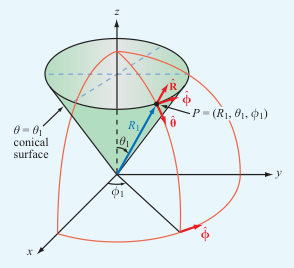
\includegraphics[width=0.7\textwidth]{fig_3.png}
	\caption{The spherical coordinate system.}
	\label{fig:figure 3}
\end{figure}

\begin{figure}[h]
	\centering
	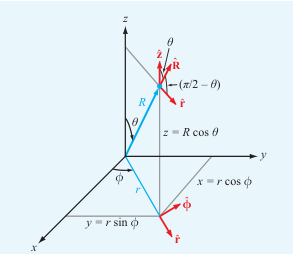
\includegraphics[width=0.6\textwidth]{fig_4.png}
	\caption{Mapping the spherical coordinate system onto the rectangular coordinate system.}
	\label{fig:figure 4}
\end{figure}

\section{Week 2: Vector Calculus}
\subsection{Differential Vectors}
In vector calculus, the infintesimal quantity \(dx\) found in single-variable calculus has a straightforward analogue: the differential length vector \(dl\). Since we're working in three dimensions, we may specify three differential length vectors \(dl_x, dl_y\) and \(dl_z\), which correspond to infinitesimal changes in position along each of their respective coordinate axes.

Making use of these three differential length vectors, we can describe a differential area vector \(ds\), whose magintude is defined as the product of two differential length vectors. For example, the differential area vector \(ds_x\) points away from the y-z plane, and is defined as \(\hat{\alpha_x}\space dydz\); in other words, it defines a vector that points in the x direction, with a magnitude defined by the product of \(dl_y\) and \(dl_z\). An analogous differential volume is defined as the product of all three differential lengths, \(d \mathcal{V} = dxdydz\). The same formulae can be derived in the other two coordinate systems (see the textbook Appendix for specific conversions).

Again, as in single-variable calculus, these differential quantites can be used to integrate along a path described by a function; only in this case we will be using multivariate functions. For example, we can derive the formula for the circumference of a circle in terms of its radius, \(C = 2\pi r\) by making use of differential length vectors in cylindrical coordinates, as follows: \[
	C = \int_{0}^{2\pi}dl_{\phi} = \int_{0}^{2\pi}rd\phi = r \int_{0}^{2\pi}d\phi = 2\pi r.
\]
Similarly, differential length, surface, and volume vectors may be used to more easily find integrals in three dimensions pertaining to objects in rectangular, cylindrical, and spherical coordinate systems.

Another group of fundamental operations in vector calculus are the gradient (del), divergence, and curl operators. 

The gradient or del operator	\(\nabla\) operates on a scalar-valued function, and outputs a vector-valued function (also known as a vector field). At each point in the resultant vector field, the gradient provides the direction and magnitude of maximum change, and is defined as \[\nablaf(x,y,z) = \hat{\alpha_x}\frac{\partial f}{\partial x} + \hat{\alpha_y}\frac{\partial f}{\partial y} + \hat{\alpha_z}\frac{\partial f}{\partial z}.\]

The divergence operator \(\nabla \cdot \) takes in a vector-valued function and outputs a scalar-valued function that quantifies the rate at which the input vector field flows outward or inward with respect to a chosen point, and is defined as \[\nabla \cdot \vec{A} = \frac{\partial A_x}{\partial x} + \frac{\partial A_y}{\partial y} + \frac{\partial A_z}{\partial z}.\]

\end{document}
